\section{Sound Recording}
For soundrecording 3 I2S (Inter-Integrated-Circuit-Sound) MEMS (Micro-Electro-Mechanical-System) microphones are used \cite{DFRobot_Fermion_I2S_MEMS_Microphone}, as they have the ability to share the same clock, ensuring that the samples are taken at the same time, which later can be compared to find the phase difference between the signals. Since the microphones use I2S, an interface is needed to interact with the microphones, but unfortunately the Raspberry Pi only has one I2S interface. A single I2S interface can be used to handle 2 microphones, by using both the left and right channels which are normally used for stereo sound. To be able to use more than 2 microphones an ESP32 is used, as it has 2 I2S interfaces, allowing it to handle up to 4 microphones, but in this case only 3 are used, resulting in 1 stereo and 1 mono.

The I2S protocol requires 3 lines \cite{ESP32_I2S}: \newline
1. SCK: Serial Clock, used to synchronise the data transmission. \newline
2. WS: Word Select, used to choose whether the left or right channels is being transmitted. \newline
3. SD: Serial Data, the actual audio data being transmitted.

These 3 channels are required for the I2S communication. 3 additional wires are used for the microphones which include 3v3 (3.3 Volt), GND (Ground) and a L/R (Left/Right) pin which is used to choose whether the microphone uses the left or right channel.

By configuring one of the I2S interfaces on the ESP32 to be the master and the other to be the slave, the clock lines can be connected, that being SCK and WS, allowing both interfaces to use the same clock. This ensures that the samples are taken at the same time, allowing for phase comparison between all 3 microphones.

When the microphones send data to the specified data pins on the ESP32, the data is written directly into a DMA (Direct Memory Access) buffer, allowing for efficient data transfer without the need for CPU intervention. The ESP32 has a DMA controller which handles the transfer of data to its buffers.
By supplying multiple DMA buffers to an I2S interface, the data can be streamed into one of the DMA buffers, while the CPU reads the previous buffers.

The resolution of the microphones can be set, and for this use case is set to 16 bits, meaning that each sample is represented by 2 bytes. When the master outputs its clock, the microphones, listen to the WS line, and depending on whether it is configured as left or right, outputs the most significant bit first, followed by the remaining bits.
The protocol can be seen in \cref{fig:I2S_protocol}.
\begin{figure}[H]
    \centering
    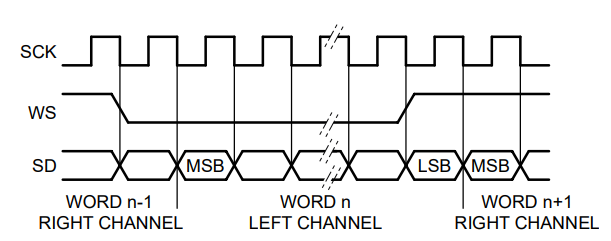
\includegraphics[width=0.7\linewidth]{Pictures/I2S_protocol.png}
    \caption{I2S protocol \cite{NXP_UM11732}}
    \label{fig:I2S_protocol}

\end{figure}

By having a higher samplerate it would be possible to increase the amount of samples which can be used to determine the phase difference between the signals. This should result in more precise calculations, but would also increase the amount of data needed to be processed by the ESP32. If the ESP32 is not fast enough to proccess the data and send it to the Raspberry Pi before the next data arrives, the DMA buffers would overflow, resulting in loss of data. The loss of data would correspond to the size of the buffer, so in this case it would be 960 samples. If an unhandled overflow occurs, the next buffer would be off by 960 samples. Later when the phase is calculated, the samples would be off by 960 samples. 

The ESP32 offers a solution of a callback \cite{ESP32_I2S}, which can be set and called when the DMA buffers overflow. It takes place in a ISR (Interrupt-Service-Routine), and the ESP32 therefore requires the callback to be placed in the IRAM (Instruction Random Access Memory), and any object passed as the arguments to the function, must be placed in the DRAM, (Data Random Access Memory). The I2S interface can therefore have a counter which increases for every filled DMA buffer, and when a DMA buffer overflows. To decrease the chance of a DMA buffer overflowing, the 2 cores on the ESP32 are utilized, making 1 core handle the I2S data recieving, stamping, and the other core handle the transfer of the data to the Raspberry Pi. % For communicating between the cores, an array of 10 buffers for data are creating globally and a queue holding the index of the current DMA buffers is used to tell the other core which buffers are ready. By making the queue one smaller than the amount of global buffers, it ensures the "writer" core will not overwrite any data before it has been sent to the computer.

\subsection{Communication with the Raspberry Pi}
The hardware on the Raspberry Pi can only work as the master on the SPI bus, and therefore the ESP32 needs to be in slave mode \cite{BCM2711_Peripherals}. Since it is the ESP32 that knows when the data is ready to be sent, a GPIO pin is used as a ``data ready'' signal form the ESP32 to the Raspberry Pi. The SPI also works with the DMA buffers, so when the ESP32 wants to use SPI to send data, two buffers can be setup, 1 for transmit and 1 for recieve. When the buffers are ready the ``data ready'' pin can be set high. The SPI offers a callback which is called when the ESP32 has loaded the DMA buffers, and is ready for a transaction, and another callback when the transaction is complete. In this callback the ``data ready'' pin can be set high and low respectively. On the Raspberry Pi an event can be set on the ``data ready'' pin on the rising edge, and when the event is triggered the Raspberry Pi can start the SPI transaction to recieve the data from the ESP32. This method makes it so the ESP32 is in charge of when the data is sent, despite being the slave in the SPI bus. 

\subsection{Electronics}
The wiring diagram can be seen in \cref{fig:ESP32_electronic}, where the microphones are connected to the I2S interfaces on the ESP32, and the pins used for SPI is also shown. The microphones are powered by the 3v3 pin on the ESP32, and GND is connected to common ground. The SEL pins are used to choose whether the microphone use the left or right channel, where microphone 1 and 2 are set to left and right respectively, and microphone 3 is set to left as it is the only one on the second I2S interface.
\begin{figure}[H]
    \centering
    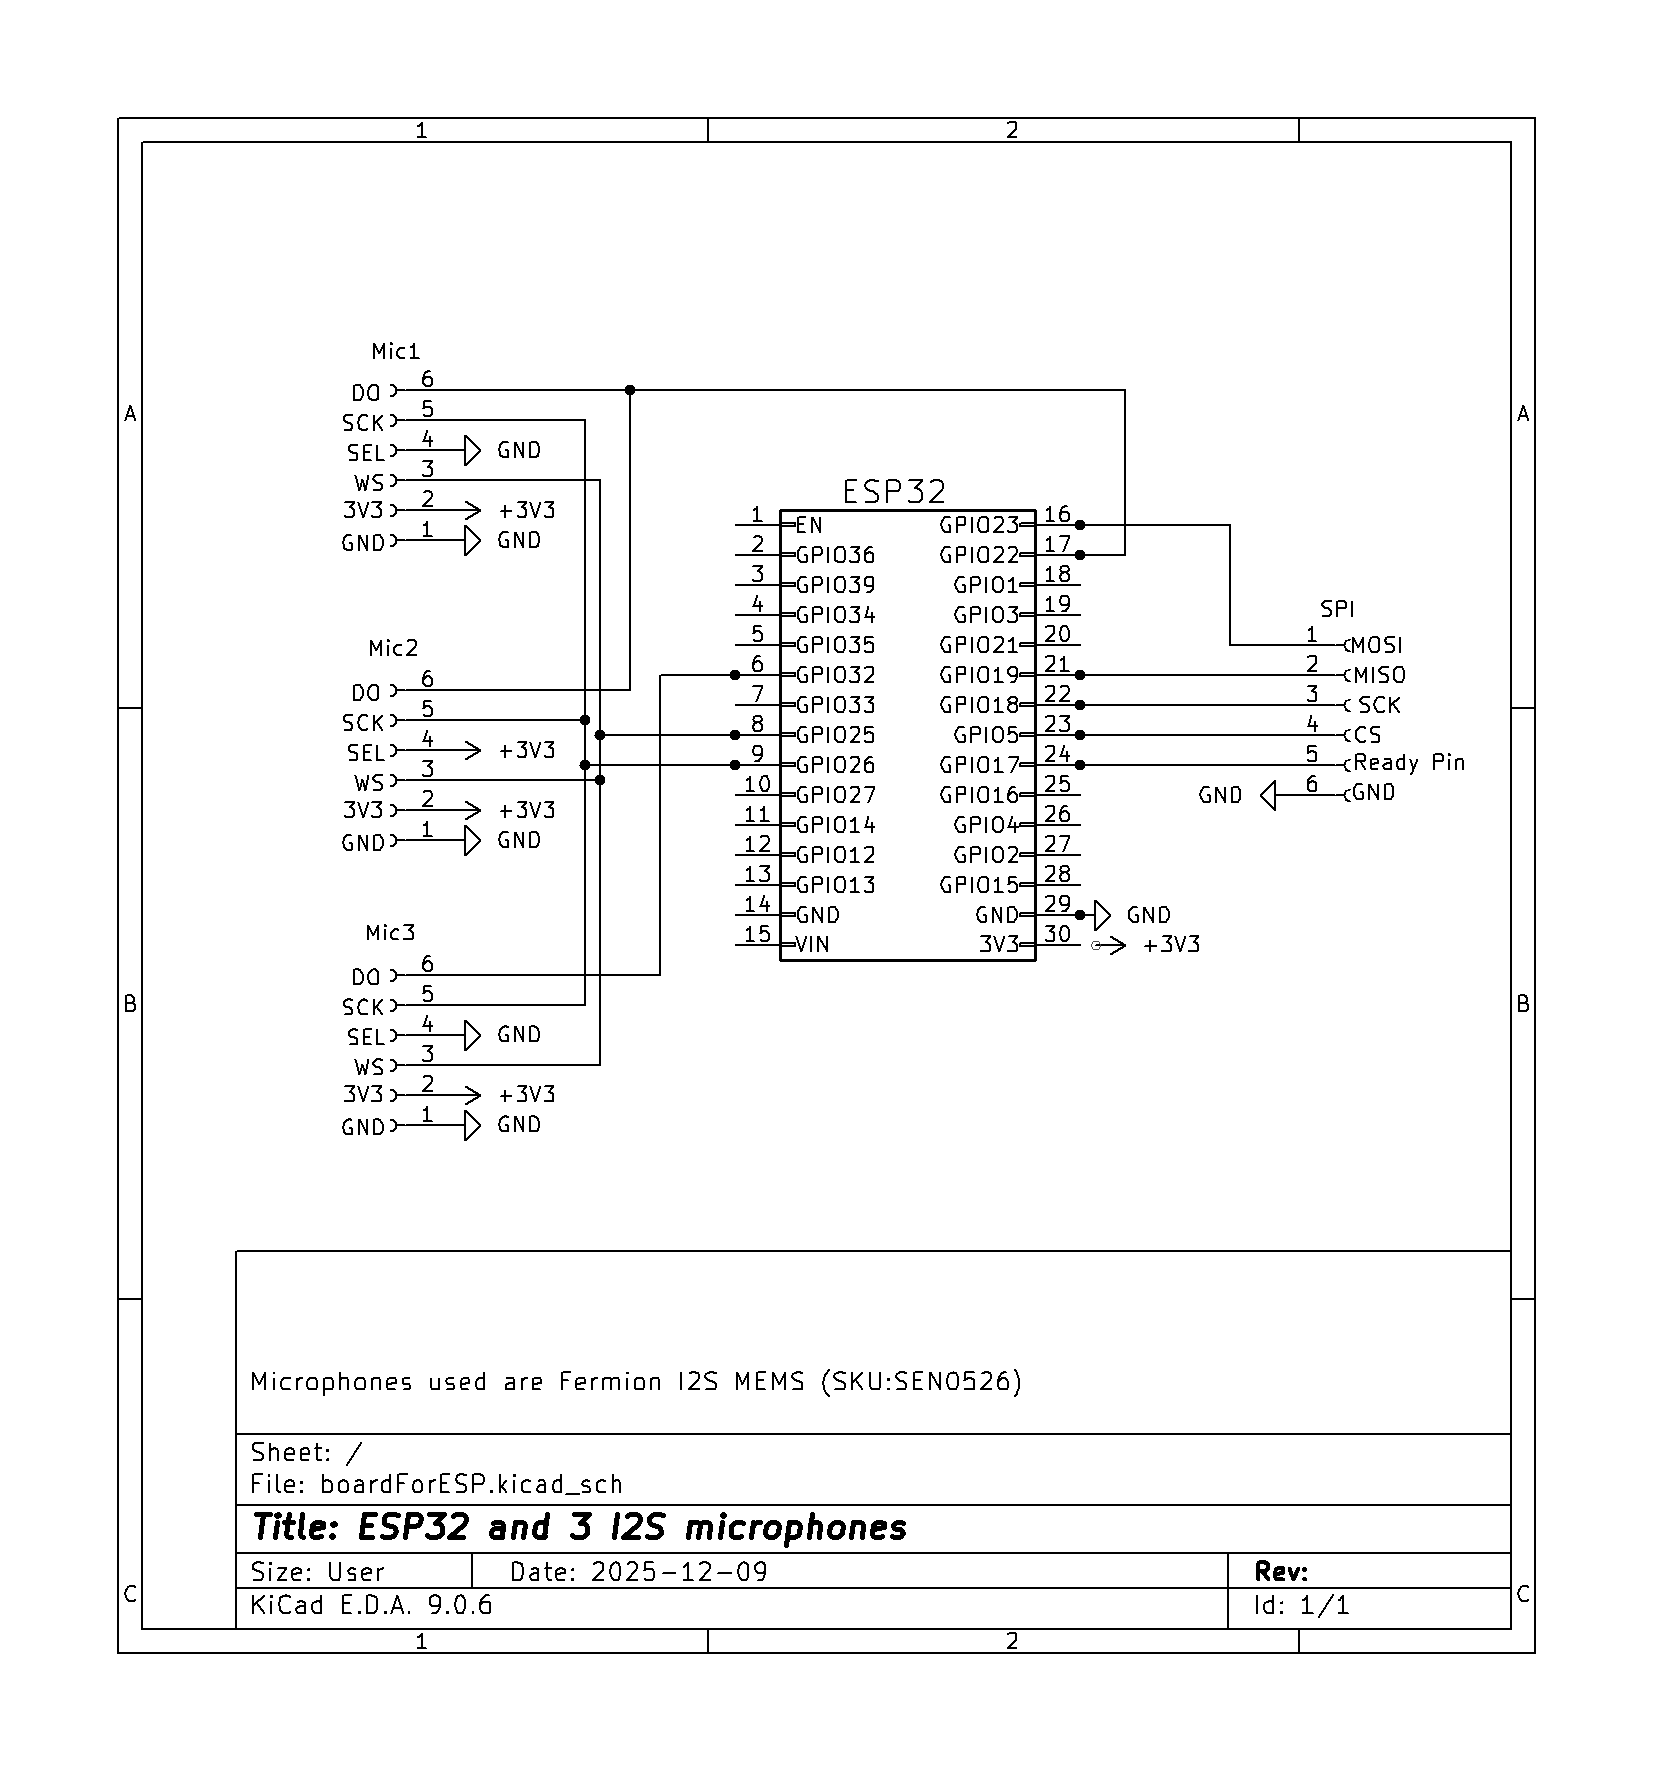
\includegraphics[width=0.7\linewidth]{Pictures/ESP32_electronic.png}
    \caption{Electrical diagram of ESP32 and microphones}
    \label{fig:ESP32_electronic}
\end{figure}